\chapter{Vorbereitung}

\section{Technische Grundlagen}

Zur Untersuchung optischer Phänomene müssen umfangreiche experimentelle Aufbauten
mit komplizierten Geräten verwendet werden. Hier soll kurz in die für diesen
Versuch notwendige Technik eingeführt werden.


    \subsection{Halbleiter}

Den Halbleiter zeichnet eine Bandlücke zwischen \emph{Valenzband} und 
\emph{Leitungsband} aus, das kleiner ist als beim Isolator, aber groß genug,
um sich vom Leiter abzugrenzen, siehe Abbildung \ref{abb:band}.
In der Technik findet sich der Halbleiter inzwischen überall.
Auch in diesem Experiment wird der Halbleiter Verwendung finden. \par
\begin{figure}[h]
  \begin{subfigure}{0.3\textwidth}
    %\centering
    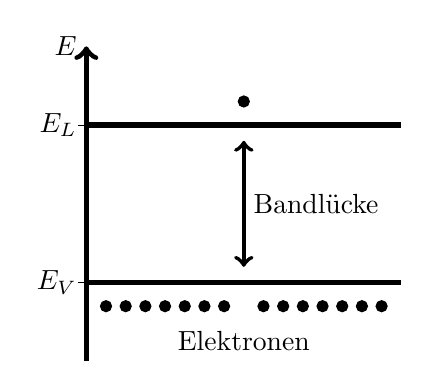
\begin{tikzpicture}
%Achse 
	\draw[draw=black,line width=2pt,->] (0,0) -- (0,4);
	\draw (-0.1,1) -- (0.1,1);
	\draw (-0.1,3) -- (0.1,3);
%Beschriftung
	\draw (0,1) node 
	  [anchor=east]
	  {$E_V$};
  \draw (0,3) node 
	  [anchor=east]
	  {$E_L$};
	\draw (0,4) node
		[anchor=east]
		{$E$};
%Bänder
	\draw[draw=black,line width=2pt] (0,1) -- (4,1);
  \draw[draw=black,line width=2pt] (0,3) -- (4,3);
	%\draw (4,1) node
	%	[anchor=west]
	%	{Valenzband};
	%\draw (4,3) node
	%	[anchor=west]
	%	{Leitungsband};
%Elektronen im Band
  \foreach \x in {1,2,...,7,9,10,...,15}{
	  \filldraw (\x/4,0.7) circle (2pt);}
	\filldraw (2,3.3) circle (2pt);
	\draw (2,0.5) node
		[anchor=north]
		{Elektronen};
%Bandlücke
	\draw[line width=1.5pt,<->] (2,1.2) -- (2,2.8);
	\draw (2,2) node
	  [anchor=west]
		{Bandlücke};
\end{tikzpicture}


  \end{subfigure}
  \begin{subfigure}{0.7\textwidth}
    %\centering
    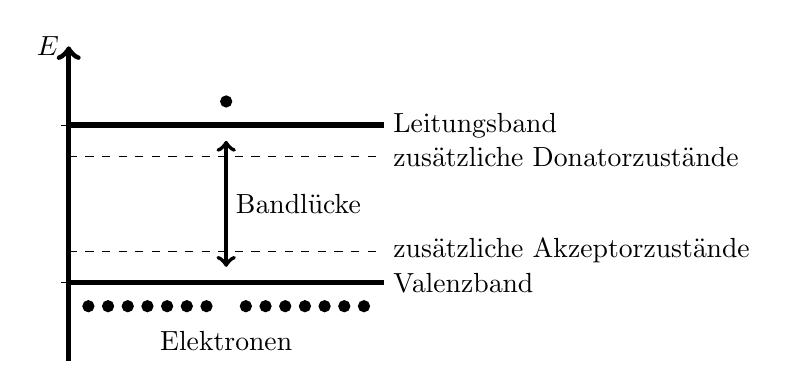
\begin{tikzpicture}
%Achse 
	\draw[draw=black,line width=2pt,->] (0,0) -- (0,4);
	\draw (-0.1,1) -- (0.1,1);
	\draw (-0.1,3) -- (0.1,3);
%Beschriftung
	%\draw (0,1) node 
	%  [anchor=east]
	%  {$E_V$};
  %\draw (0,3) node 
	%  [anchor=east]
	%  {$E_L$};
	\draw (0,4) node
		[anchor=east]
		{$E$};
%Bänder
	\draw[draw=black,line width=2pt] (0,1) -- (4,1);
  \draw[draw=black,line width=2pt] (0,3) -- (4,3);
	\draw (4,1) node
		[anchor=west]
		{Valenzband};
	\draw (4,3) node
		[anchor=west]
		{Leitungsband};
%Elektronen im Band
  \foreach \x in {1,2,...,7,9,10,...,15}{
	  \filldraw (\x/4,0.7) circle (2pt);}
	\filldraw (2,3.3) circle (2pt);
	\draw (2,0.5) node
		[anchor=north]
		{Elektronen};
%Bandlücke
	\draw[line width=1.5pt,<->] (2,1.2) -- (2,2.8);
	\draw (2,2) node
	  [anchor=west]
		{Bandlücke};
%Donator- und Akzeptorzustände
	\draw[dashed] (0,1.4) -- (4,1.4);
	\draw (4,1.4) node
		[anchor=west]
		{zusätzliche Akzeptorzustände};
	\draw[dashed] (0,2.6) -- (4,2.6); 
	\draw (4,2.6) node
		[anchor=west]
		{zusätzliche Donatorzustände};
\end{tikzpicture}

  \end{subfigure}
  \caption{Bandstrukturen eines (a) reinen Halbleiters, (b) dotierten Halbleiters}
  \label{abb:band}
\end{figure}
In der Technik werden Halbleiter meist \emph{dotiert}. Hierbei werden gezielt 
Fremdatome in das Gitter eingebracht, um so das Verhältnis von Lochdichte zu
Elektronendichte zu manipulieren. \emph{Donatoren} geben Elektronen an das Gitter 
ab, während \emph{Akzeptoren} diese aufnehmen und so ein zusätzliches Loch 
schaffen. Da die Bindungsenergie des Donators kleiner als die Bandlücke ist, entstehen
zusätzliche Niveaus, die energetisch etwas tiefer liegen, als das Leitungsband.
Beim Akzeptor entstehen neue Niveaus etwas oberhalb des Valenzbandes, siehe 
Abbildung \ref{abb:band}.
Bringt man nun zwei gegensätzlich dotierte Halbleiter in Kontakt, das mit Donatoren
dotierte Gebiet nennt man n-Typ, das mit Akzeptoren dotierte p-Typ, so entsteht an
der Grenzfläche der \emph{pn-Übergang}, siehe Abbildung \ref{abb:pn}.
\begin{figure}[h]
  \centering
  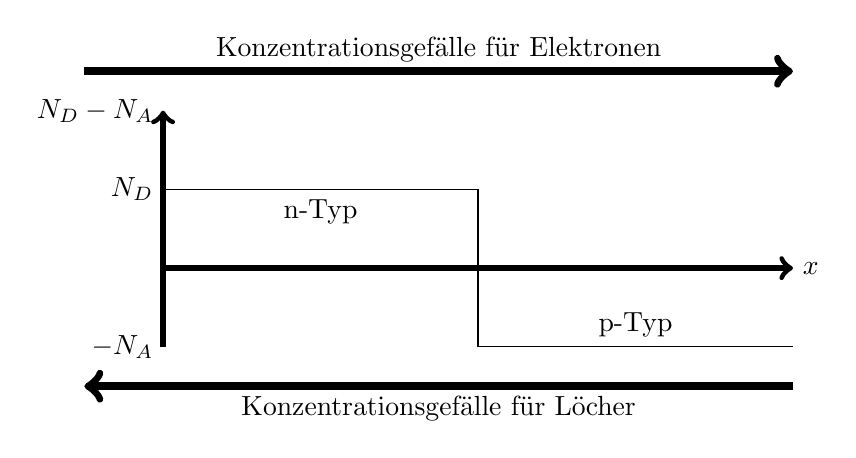
\begin{tikzpicture}
%Achsen
  \draw[line width=2pt,->] (0,0) -- (0,3);
  \draw (0,3) node
    [anchor=east]
    {$N_D - N_A$};
  \draw[line width=2pt,->] (0,1) -- (8,1);
  \draw (8,1) node
    [anchor=west]
    {$x$};
%Gefälle
  \draw[line width=3pt,->] (-1,3.5) -- (8,3.5);
  \draw (3.5,3.5) node
    [anchor=south]
    {Konzentrationsgefälle für Elektronen};
  \draw[line width=3pt,->] (8,-0.5) -- (-1,-0.5);
  \draw (3.5,-0.5) node
    [anchor=north]
    {Konzentrationsgefälle für Löcher};
%Graph
  \draw (0,2) node
    [anchor=east]
    {$N_D$};
  \draw (0,0) node
    [anchor=east]
    {$-N_A$};
  \draw (0,2) -- (4,2);
  \draw (2,2) node
    [anchor=north]
    {n-Typ};
  \draw (4,2) -- (4,0);
  \draw (4,0) -- (8,0);
  \draw (6,0) node
    [anchor=south]
    {p-Typ};
\end{tikzpicture}


  \caption{Konzentration von Donatoren und Akzeptoren. $N_D$ beschreibt hier die
           Donatorkonzentration, $N_A$ die Akzeptorkonzentration.}
  \label{abb:pn}
\end{figure}
Durch die unterschiedlichen Dotierungen entsteht in Richtung des p-dotierten Gebiets
ein Konzentrationsgefälle für Elektronen, während in Richtung des n-dotierten 
Gebiets ein Gefälle der Löcherkonzentration entsteht. Dies führt zu einem
Elektronenstrom in das p-, und einem Löcherstrom in das n-Gebiet. Die Folge dieser
Ströme ist eine Verarmung an beweglichen Ladungsträgern im Gebiet um den 
Übergang. Da die Ionen, Donatoren und Akzeptoren, nicht mehr durch freie Elektronen
und Löcher kompensiert werden, entsteht ein Gebiet mit positiven/negativen
Raumladung. Dieses Gebiet wird \emph{Raumladungszone} genannt. Legt man an den
pn-Übergang eine Spannung an, kann man die typische Diodenkennlinie beobachten.
Diese ist in Abbildung \ref{abb:diodui} zu sehen.
Der pn-Übergang ist also Basis für den Großteil der modernen Technologie.
\begin{figure}
  \centering
  %\scalebox{0.55}[0.49]{\import{Abb/}{diodenkennlinie.pdf_tex}}
    \scalebox{0.9}{\import{Abb/}{diodenkennlinie_gestaucht.pdf_tex}}
  \caption{Qualitative Darstellung einer Diodenkennlinie \autocite{wiki:diode}}
  \label{abb:diodui}
\end{figure}

\clearpage

    \subsection{Photodiode}

Betrachtet man einen solchen pn-Halbleiter unter Lichteinfall, kann man den 
\emph{photoelektrischen Effekt} beobachten. Photonen mit einer Energie 
$E= h \cdot \nu$ können Elektronen ins Leitungsband anregen,
falls $h \cdot \nu > E_g$, mit der Größe der Bandlücke $E_g$.
Dies wird in Abbildung \ref{abb:photo} veranschaulicht.
\begin{figure}[h]
  \centering
  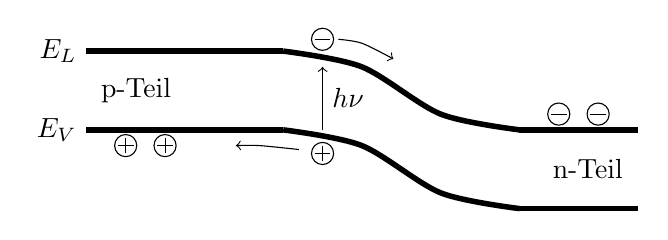
\begin{tikzpicture}
%Bänder
  \draw[line width=2pt] (0,2) -- (2.5,2);
  \draw[line width=2pt] plot [smooth] coordinates {(2.5,2) (3.5,1.8) (4.5,1.2) (5.5,1)};
  \draw[line width=2pt] (5.5,1) -- (7,1);
  \draw (0,2) node 
    [anchor=east]
    {$E_L$};
  \draw[line width=2pt] (0,1) -- (2.5,1);
  \draw[line width=2pt] plot [smooth] coordinates {(2.5,1) (3.5,0.8) (4.5,0.2) (5.5,0)};
  \draw[line width=2pt] (5.5,0) -- (7,0);
  \draw (0,1) node 
    [anchor=east]
    {$E_V$};
%Beschriftung
  \draw (1.2,1.5) node
    [anchor=east]
    {p-Teil};
  \draw (5.8,0.5) node
    [anchor=west]
    {n-Teil};
%Teilchen
  \draw (3,2.15) circle (4pt);
  \draw (2.9,2.15) -- (3.1,2.15);
  \draw (6,1.2) circle (4pt);
  \draw (5.9,1.2) -- (6.1,1.2);
  \draw (6.5,1.2) circle (4pt);
  \draw (6.4,1.2) -- (6.6,1.2);
  \draw[->] plot [smooth] coordinates {(3.2,2.15) (3.5,2.1) (3.9,1.9)};

  \draw (3,0.7) circle (4pt);
  \draw (2.9,0.7) -- (3.1,0.7);
  \draw (3,0.6) -- (3,0.8);
  \draw (1,0.8) circle (4pt);
  \draw (0.9,0.8) -- (1.1,0.8);
  \draw (1,0.7) -- (1,0.9);
  \draw (0.5,0.8) circle (4pt);
  \draw (0.4,0.8) -- (0.6,0.8);
  \draw (0.5,0.7) -- (0.5,0.9);
  \draw[->] plot [smooth] coordinates {(2.7,0.75) (2.2,0.8) (1.9,0.8)};

  \draw[->] (3,1.0) -- (3,1.8);
  \draw (3,1.4) node
    [anchor=west]
    {$h\nu$};
\end{tikzpicture}


  \caption{Anregen eines Elektrons im pn-Übergang}
  \label{abb:photo}
\end{figure}
Im Bereich des pn-Übergangs werden weitere Elektronen ins Leitungsband angeregt.
Wie im vorherigen Abschnitt besprochen entstehen im p-Teil zusätzliche 
Akzeptorzustände über dem Valenzband und im n-Teil zusätzliche Donatorzustände
unter dem Leitungsband. Der Bandverlauf ist, wie in Abbildung \ref{abb:photo} 
zu sehen, um den pn-Übergang gebogen. Nach der Anregung diffundiert das Elektron
in den n-Teil, da hier ein Mangel an beweglichen Elektronen herrscht, während das
Loch in den p-Teil driftet. Dies führt zu einer Photospannung, die am Halbleiter
abgenommen werden kann.


    \subsection{Laser}

Der Laser (\f light \f amplification by \f stimulated \f emission of \f radiation)
ist eine Lichtquelle, die sich durch hohe Strahlungsintensität, einen engen 
Frequenzbereich, starker Bündelung des Strahls und einer großen Kohärenzlänge 
auszeichnet. \par
\begin{figure}[h]
  \centering
  \import{Abb/}{emission.pdf_tex}
  \caption{Wechselwirkung zwischen Photonen und Elektronen im Atom}
  \label{abb:emission}
\end{figure}
Zur Lichterzeugung wird die \emph{spontane} und \emph{induzierte Emission} 
ausgenutzt, die in Abbildung \ref{abb:emission} skizziert ist. Ein Photon kann
ein gebundenes Elektron durch \emph{Absorption} auf ein höheres Energieniveau 
heben. Selbiges kann durch \emph{spontane Emission} unter Abgabe eines Photons
zurück in das niedrigere Niveau wechseln. Trifft dieses Photon auf ein weiteres
angeregtes Elektron, so kann dieses Elektron zur Emission angeregt werden, zur
\emph{induzierten Emission}. Wichtig ist hierbei, dass alle emittierten Photonen
die gleiche Energie tragen. Das Licht ist also monochromatisch. \par
\begin{figure}
  \centering
  \import{Abb/}{aufbau_laser.pdf_tex}
  \caption{Aufbau eines Lasers}
  \label{abb:aufbau_laser}
\end{figure}
Soll mithilfe dieses Prinzips ein intensiver Strahl erzeugt werden, so müssen 
möglichst viele Elektronen in diesen angeregten Zustand gebracht werden. Hierzu
verwendet man eine \emph{Pumpquelle}, siehe Abbildung \ref{abb:aufbau_laser}.
Diese Pumpe regt im \emph{aktiven Material},
also das Material, in dem die Emission stattfinden soll, die Elektronen an, sodass
mehr Elektronen im energetisch höheren Energieband aufhalten. Dieser Zustand wird
\emph{Besetzungsinversion} genannt. Durch spontane Emission wandern erste Photonen
durch das aktive Material und induzieren weitere Emission. 
Ein \emph{optischer Resonator}, oft verwirklicht durch zwei Spiegel, reflektiert nun
die Photonen immer wieder zurück in das aktive Material, wodurch sich eine stehende
Welle bildet. Der vordere Spiegel lässt immer einen Teil der Strahlung entweichen.
So entsteht ein homogener, intensiver Strahl. \par
Zur Versuchsdurchführung wird eine besondere Bauart des Lasers verwendet, der 
\emph{Faserlaser}. Dieser gibt statt einem kontinuierlichen Strahl kurze Pulse ab.
Der Aufbau ist hier komplexer, siehe Abbildung \ref{abb:faser}.
Das aktive Medium ist eine Erbium-dotierte Glasfaser. Durch eine Leuchtdiode, in der
Abbildung \emph{Pump Diode}, wird eine Besetzungsinversion der Erbium-Ionen
hergestellt. An den Enden der Faser bilden zwei teildurchlässige Spiegel den 
Resonator. Durch einen sättigbaren Absorber, \emph{SAM}, der nur kurze intensive
Impulse transmittiert, wird der gepulste Charakter des Lasers erreicht. Nach dem 
Verlassen des Oszillators erfolgt eine weitere Verstärkung in einer dotierten 
Glasfaser, wieder durch eine Diode gepumpt, bevor der Impuls ausgesendet wird. 
Daraus wird eine Pulsenergie von ~$\SI{0,8}{eV}$ erreicht.
Eine interessante Folge des gepulsten Charakters mit derart hohen Energien findet
sich in der Pulsform des Lasers. Anstatt eines monochromatischen Spektrums, wie 
man es von Lasern erwarten würde, hat der Laser eine breitere
Wellenlängenverteilung. Dies ist mit der Energie-Zeit Unschärfe zu begründen.
Durch die hohen Energien ist die Zeit nicht mehr scharf genug aufgelöst, um 
eine schmale Wellenlängenverteilung zu erreichen.
\autocite{phying, zinth}
\begin{figure}[H]
  \centering
  \import{Abb/}{faserlaser.pdf_tex}
  \caption{Aufbau eines Faserlasers}
  \label{abb:faser}
\end{figure}


    \subsection{Lock-In Verstärker}

In der Experimentalphysik arbeitet man oft mit Messsignalen, die um ein 
vielfaches schwächer sind, als das Umgebungsrauschen, das unweigerlich
Auftritt. Ohne passende Verstärkung und Filterung sind diese Messungen wertlos.
Abhilfe schafft in diesem Experiment der Lock-In Verstärker. 
\begin{figure}[hb]
  \centering
  \import{Abb/}{lockin.pdf_tex}
  \caption{Signalverarbeitung mit einem Lock-In Verstärker}
  \label{abb:lockin}
\end{figure}
Die Funktion des Verstärkers erkennt man am besten anhand eines Signals. In 
Abbildung \ref{abb:lockin} ist eine rein qualitative Darstellung eines möglichen
Messsignals abgebildet. Das Signal selbst ist durch das starke Rauschen kaum zu
erkennen. Im ersten Schritt wird ein Hochpass angewandt. Das kräftige Rauschen
gegen $\SI{0}{Hz}$ fällt dadurch weg. Danach wird eine sehr enger Bandpass um
das eigentliche Signal angewandt. Die ungefähre Frequenz ist bei vielen Anwendungen
bekannt. Beispiele sind die Herzfrequenz, oder wie in diesem Experiment die 
Frequenz der Lichtquelle. So wird ein Großteil des Rauschen gefiltert, in der 
Abbildung schraffiert, und das Signal kann weiter ausgewertet werden.

    \subsection{Pump-Probe Versuch}

Zur Untersuchung der Ladungsträgerdynamik in InGaAs wird ein sogenannter Pump-Probe Versuch verwendet. Hierbei wird die Probe (in unserem Fall der InGaAs Kristall) zunächst von einem leistungsstarken Pumppuls angeregt und anschließend von einem schwächeren Abtastpuls durchlaufen, welcher schließlich auf eine Photodiode trifft. Die Transmission des Abtastpulses hängt nun davon ab, wie viele Elektronen sich im angeregten Zustand befinden, bzw. anders ausgedrückt: wie viele Photonen noch absorbiert werden können. Trägt man nun die transmittierte Intensität des Abtastpulses gegen die Verzögerungszeit $\tau$ zwischen dem Auftreffen der beiden Pulse auf, so kann beobachtet werden, wie sich die Ladungsträger der Probe im angeregten Zustand verhalten: Bei einer Verzögerungszeit von $\tau<0$ trifft der Abtastpuls auf eine noch nicht angeregte Probe, d.h. hier findet die minimale Transmission statt. Bei $\tau=0$ steigt die Transmission stark an, da der Pumppuls nun schon Elektronen angeregt hat und der Abtastpuls somit weniger absorbiert wird. Bei $\tau>0$ sinkt die Transmission mit steigender Verzögerungszeit wieder, da in der Zeit zwischen Anregung durch den ersten Puls und Eintreffen des zweiten Pulses schon wieder Elektronen ins Valenzband rekombiniert sind.

In diesem Versuch entstehen Pump- und Abtastpuls dadurch, dass ein Laserpuls durch einen $97:3$ Strahlteiler in einen starken und einen schwachen Puls aufgeteilt werden.      

\autocite{Diels2006}

\section{Nichtlineare Optik}
    \subsection{Doppelbrechung}

Um das Prinzip der Doppelbrechung verstehen zu können, gilt es zunächst die 
Polarisation des Lichts zu verstehen. Hierzu betrachten wir zunächst die 
Eigenschaften einer elektromagnetischen Welle.\par
Aus den Maxwellgleichungen lässt sich die Transversalität der elektromagnetischen
Welle zeigen, der Wellenvektor $\vec{k}$ steht also senkrecht zum elektrischen 
Feld $\vec{E}$. Für eine Welle die sich in z-Richtung ausbreitet, gilt also
\[
    \vec{E} = \vec{E}_x + \vec{E}_y = 
      \begin{pmatrix}
          E_{x0} \cos(kz-\omega t)\\
          E_{y0} \cos(kz-\omega t + \epsilon)\\
          0
      \end{pmatrix}
\]
Das $\epsilon$ beschreibt hierbei die Phasendifferenz der Feldkomponenten.

Diese Betrachtung lässt nun einige wichtige Polarisationszustände zu.\\
\textbf{Linear polarisiert:} Für die Fälle $\epsilon = \pm 2n \, \pi$ und
$\epsilon = (2n+1) \pi$ sind die Komponenten $\vec{E}_x$ und $\vec{E}_y$ in bzw.
außer Phase. Dies führt zu einer zeitlich konstanten Feldrichtung.
\[
    \vec{E} = 
      \begin{pmatrix}
          E_{x0}\\
          E_{y0}\\
          0
      \end{pmatrix}
    \cos (kz-\omega t) = \vec{E}_0 \cos (kz-\omega t)
\]
\textbf{Zirkular polarisiert:} Ist nun $E_{x0} = E_{y0} = E_0$ mit 
$E = | \vec{E} |$ und $\epsilon = \frac{\pi}{2} + m \pi$, $m \in N_0$, so beschreibt
die Drehung der Feldrichtung über die Zeit einen Kreis in der x-y Ebene. Es gilt
\[
    \vec{E} = E_0
        \begin{pmatrix}
            \cos(kz-\omega t)\\
            \pm \sin(kz-\omega t)
            0
        \end{pmatrix}
\]

Für alle anderen Fälle ist das Licht \textbf{elliptisch polarisiert}. Die 
Drehung der Feldrichtung beschreibt eine Ellipse in der x-y Ebene.

Diese Eigenschaft findet zum Beispiel in Polarisatoren und Analysatoren Anwendung.
Es gibt Materialien, die nur Licht einer bestimmten Polarisationsrichtung
transmittieren. So spricht man von einem Linear-, Zirkular-, oder einem elliptischen
Polarisator. Verwendet man zwei Polarisatoren nacheinander, so spricht man von 
einem Analysator.
Aus der Quelle wird mithilfe des ersten Polarisator nur eine bestimmte
Richtung transmittiert. Den zweiten gleichartigen Polarisator kann man 
dann um einen Winkel $\Theta$ verdrehen, sodass nur noch ein Teil des Lichts
transmittiert wird. Wird er um $90^\circ$ verdreht, so wird die komplette
Intensität gefilter. Quantitativ ergibt sich
\[
    I(\Theta) = I_0 \cos^2 \Theta
\]

In der linearen Optik werden Materialien betrachtet, die optisch isotrop sind.
Die Lichtausbreitung war also unabhängig von der Richtung. Es gilt
\[
    \vec{D} = \epsilon_0 \epsilon \vec{E}
\]
Die dielektrischen Eigenschaften der Medien wird durch die dielektrische
Verschiebung $\vec{D}$ berücksichtigt. Das Feld $\vec{E}$ wird durch
die dielektrische Konstante $\epsilon$ abgeschwächt. Die Richtung von 
$\vec{D}$ und $\vec{E}$ ist jedoch immer die Gleiche. 

In der nichtlinearen Optik muss dieses Konzept für nichtisotrope Medien erweitert
werden. Ein solches Medium ist bezüglich seiner dielektrischen Eigenschaften nicht
mehr symmetrisch. Die Konstante $\epsilon$ wird durch den Tensor $\epsilon_{ij}$ 
ersetzt. Dieser hat die Form
\[
    \epsilon_{ij} = 
        \begin{pmatrix}
            \epsilon_{11} \; \epsilon_{12} \; \epsilon_{13} \\
            \epsilon_{21} \; \epsilon_{22} \; \epsilon_{23} \\
            \epsilon_{31} \; \epsilon_{32} \; \epsilon_{33} \\
        \end{pmatrix}
\]
Die Gleichung $\vec{D} = \epsilon_0 \epsilon_{ij} \vec{E}$ kann man noch 
vereinfachen,
indem man die Achsen des Koordinatensystems den Hauptachsen des Kristalls angleicht.
Dadurch muss man nur die Einträge der Diagonale betrachten.
So ergibt sich für die einzelnen Richtungen
\[
    D_i = \epsilon_0 \epsilon_i E_i, \qquad i=x,y,z
\]
Mit dieser Gleichung lassen sich drei Arten von Medien unterscheiden.

\begin{enumerate}
    \item \textbf{Optisch isotrope Medien:} 
          $\epsilon_x = \epsilon_y = \epsilon_z = \epsilon$
          Die Richtung spielt also keine Rolle und man landet in der linearen Optik.

    \item \textbf{Optisch einachsige Kristalle:}
          Man setzt eine optische Achse, z.B. in z-Richtung. Für die Richtungen 
          gilt dann $\epsilon_x = \epsilon_y = \epsilon_{\bot}, \quad 
                     \epsilon_z = \epsilon_{\parallel}$
          Die Lichtausbreitung längs der optischen Achse erfolgt dann ohne
          Polarisationsabhängigkeit. Bei allen anderen Richtungen werden die 
          unterschiedlichen Polarisationsrichtungen des einfallenden Lichtes
          unterschiedlich gebrochen. Die quantitative Betrachtung erfolgt 
          später.
    \item \textbf{Optisch zweiachsige Kristalle:}
          Hier gilt $\epsilon_x \neq \epsilon_y \neq \epsilon_z \neq \epsilon_x$.
          Es gibt also zwei Achsen mit polarisationsabhängiger Lichtausbreitung.
\end{enumerate}
Für diesen Versuch besonders wichtig sind die optisch einachsigen Kristalle, die im
folgenden genauer betrachtet werden sollen.

Die Lichtausbreitung im Medium kann man mithilfe der oben Beziehung zwischen 
$\vec{D}$ und $\vec{E}$ und den Maxwellgleichungen herleiten. Daraus kann man 
für eine ebene Welle in nichtmagnetischen Substanzen folgende Relationen herleiten
\[
    \vec{D} \bot \vec{k}, \quad \vec{B} \bot \vec{k}, \quad
    \vec{B} \bot \vec{E}, \quad \vec{B} \bot \vec{D}
\]
Für den Poyntingvektor $\vec{S}$, der den Energiefluss der Welle beschreibt, 
gilt analog zur linearen Optik
\[
    \vec{S} = \frac{1}{\mu_0} \vec{E} \times \vec{B}
\]
Wie in Abbildung \ref{abb:doppel} zu sehen, breitet sich der Strahl nicht in
Richtung des Wellenvektors, sondern in Richtung des Poyntingvektors aus. In der
linearen Optik zeigen diese in die gleiche Richtung.
\begin{figure}[h]
  \centering
  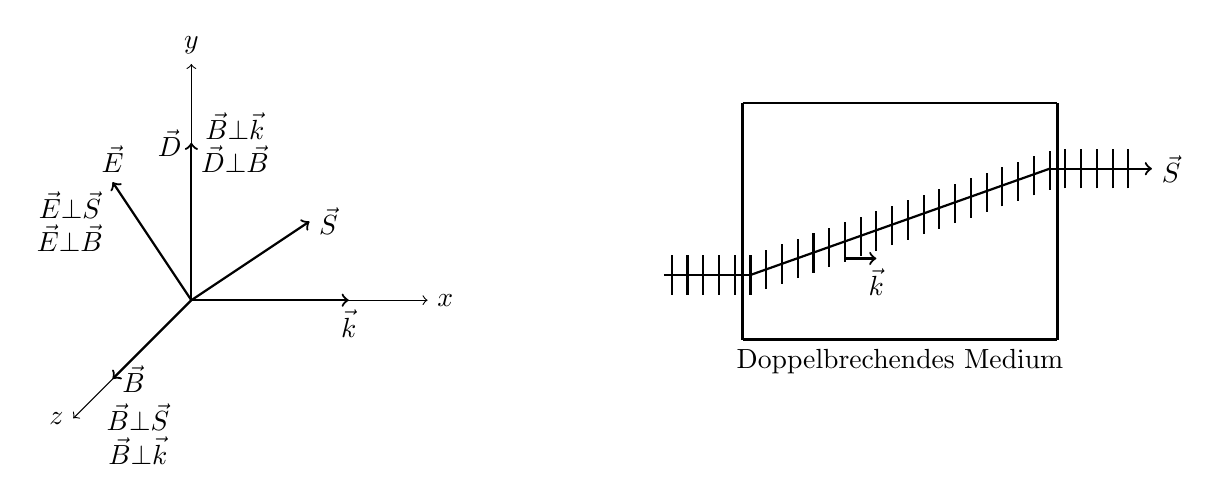
\begin{tikzpicture}[every text node part/.style={align=center}]
%Richtungen der Vektoren
    %Achsen
    \draw[->] (3,0) -- (1.5,-1.5); %z
    \draw (1.5,-1.5) node
        [anchor=east]
        {$z$};
    \draw[->] (3,0) -- (6,0);    %x
    \draw (6,0) node
        [anchor=west]
        {$x$};
    \draw[->] (3,0) -- (3,3);    %y
    \draw (3,3) node
        [anchor=south]
        {$y$};

    %Vektoren
    \draw[thick, ->] (3,0) -- (5,0);
    \draw (5,0) node
        [anchor=north]
        {$\vec{k}$};
    \draw[thick, ->] (3,0) -- (3,2);
    \draw (3,2) node
        [anchor=east]
        {$\vec{D}$};
    \draw[thick, ->] (3,0) -- (2,-1);
    \draw (2,-1) node
        [anchor=west]
        {$\vec{B}$};
    \draw[thick, ->] (3,0) -- (4.5,1);
    \draw (4.5,1) node
        [anchor=west]
        {$\vec{S}$};
    \draw[thick, ->] (3,0) -- (2,1.5);
    \draw (2,1.5) node
        [anchor=south]
        {$\vec{E}$};

    %Beschreibungen
    \draw (3,2) node
        [anchor=west]
        {$\vec{B} \bot \vec{k}$ \\ $\vec{D} \bot \vec{B}$};
    \draw (2,1) node
        [anchor=east]
        {$\vec{E} \bot \vec{S}$ \\ $\vec{E} \bot \vec{B}$};
    \draw (1.8,-1.7) node
        [anchor=west]
        {$\vec{B} \bot \vec{S}$ \\ $\vec{B} \bot \vec{k}$};

%Wellenfront im Medium
    %Rechteck
    \draw[thick] (10,-0.5) -- (10,2.5);
    \draw[thick] (14,-0.5) -- (14,2.5);
    \draw[thick] (10,-0.5) -- (14,-0.5);
    \draw[thick] (10,2.5) -- (14,2.5);
    \draw (12,-0.5) node
        [anchor=north]
        {Doppelbrechendes Medium};

    %Wellenfronten
    \foreach \x in {0,1,...,4}{
        \draw[thick] (9.1 + \x*0.2, 0.07) -- (9.1 + \x*0.2, 0.57);}
    \foreach \x in {1,2,...,20}{
        \draw[thick] (9.9 + \x*0.2, 0 + \x*0.07) -- (9.9 + \x*0.2, 0.5 + \x*0.07);}
    \foreach \x in {1,2,...,5}{
        \draw[thick] (13.9 + \x*0.2, 1.42) -- (13.9 + \x*0.2, 1.92);}
    \draw[->,thick] (11.3,0.53) -- (11.7,0.53);
    \draw (11.7,0.53) node
        [anchor=north]
        {$\vec{k}$};

    %Strahlrichtung
    \draw[thick] (9,0.32) -- (10.1,0.32);
    \draw[thick] (10.1,0.32) -- (13.9,1.67);
    \draw[->,thick] (13.9,1.67) -- (15.2,1.67);
    \draw (15.2, 1.67) node
        [anchor=west]
        {$\vec{S}$};

\end{tikzpicture}


    \caption{a) Skizze der einzelnen Vektoren einer Welle. b) Skizze der 
             Wellenausbreitung des außerordentlichen Strahls im Medium.}
  \label{abb:doppel}
\end{figure}
Für einen einachsigen Kristall lässt sich ein lineares Gleichungssystem 
aufstellen, woraus sich dann 2 Werte für den Brechungsindex $n$ bestimmen lassen.
\[
    \frac{1}{n_{ao}^2} = \frac{\cos^2(\Theta)}{\epsilon_{\bot}} +
                         \frac{\sin^2(\Theta)}{\epsilon_{\parallel}},
    \qquad n_0 = \sqrt{\epsilon_{\bot}}
\]
Hier beschreibt $n_{ao}$ den außerordentlichen Strahl, dessen Ausbreitung in
Abbildung \ref{abb:doppel} b) zu sehen ist. $n_o$ beschreibt dagegen den 
ordentlichen Strahl, der den Gesetzen der linearen Optik folgt. 
$\Theta$ ist der vom Wellenvektor $\vec{k}$ und der optischen Achse 
eingeschlossene Winkel. Für einen zur optischen Achse parallelen Strahl, 
$\Theta=0$, ergibt sich $n_0$ als einziger Brechungsindex, sodass in diesem Fall
ordentliche Strahl beobachtet werden kann.

\paragraph*{Polarisationsdreher:} Eine wichtige, auch in diesem Versuch benutzte, Anwendung	der Doppelbrechung ist der Polarisationsdreher, oft einfach "$\lambda/2$-Plättchen"{} genannt. Es besteht meist aus einer dünnen Schicht eines doppelbrechenden Materials (z.B. Kalkspat) und kann dazu verwendet werden, die Polarisationsrichtung von linear polarisiertem Licht um einen beliebigen Winkel zu drehen: Fällt eine elektromagnetische Welle mit einer zur optischen Achse des $\lambda/2$-Plättchens um den Winkel $\alpha$ geneigten Polarisation ein, so wird diese beim Durchlaufen des Polarisationsdrehers um den Winkel $2\alpha$ gedreht. Der Effekt kommt dadurch Zustande, dass sich nach Durchlaufen des Plättchens zwischen dem zur optischen Achse parallelen und senkrechten Polarisationsanteil eine Phasendifferenz von $\lambda/2$ ergibt, welche in der entsprechenden Drehung der Polarisation resultiert. Der Prozess ist in Abb. \ref{lambda_halbe} veranschaulicht.

In diesem Versuch wird der Polarisationsdreher in Kombination mit einem Polfilter verwendet, wodurch es möglich ist, die Intensität des Pumpstrahls stufenlos einzustellen ohne dabei dessen Polarisationsrichtung zu ändern, wie im Abschnitt zum Analysator beschrieben. Für die Intensität gilt

\[I=I_{0}\, \cos^2(\alpha)\]

\begin{figure}[H]
	\centering
        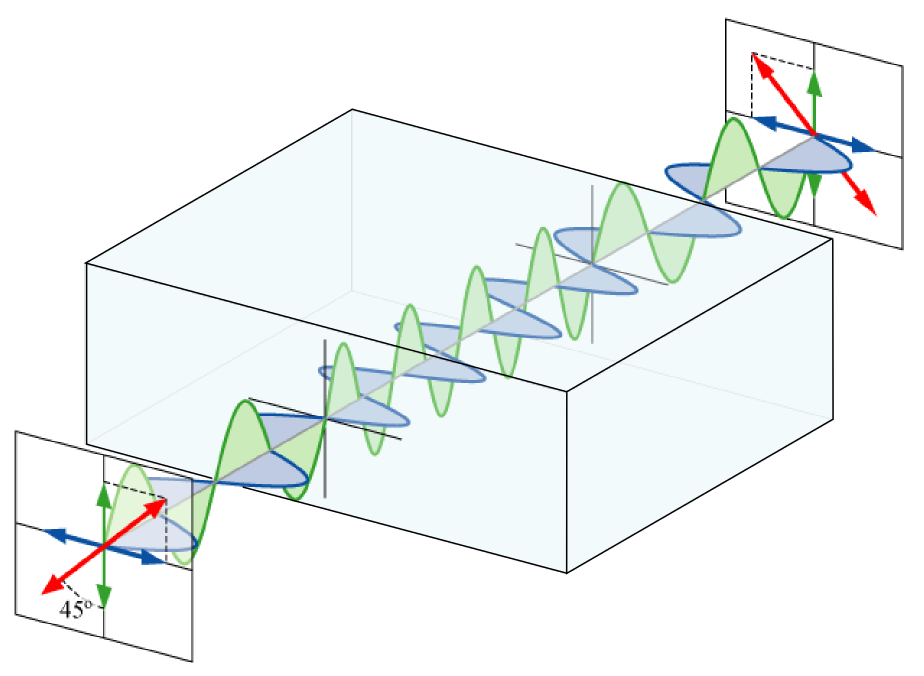
\includegraphics[width=0.8\textwidth]{Abb/lambda_halbe.png}
        \caption{Veranschaulichung des im Polarisationsdreher ablaufenden Prozesses. Die Polarisation der Welle ist als roter Pfeil dargestellt, die optische Achse des $\lambda/2$-Plättchens in grün.\autocite{wiki:lambdahalbe}}
	\label{lambda_halbe}
\end{figure}

\autocite{zinth}, \autocite{hecht}, \autocite{demtroeder}

    \subsection{Phasenanpassung}

Eine weitere Anwendung der Doppelbrechung in diesem Versuch findet sich in der
Phasenanpassung.

Durch die Frequenzabhängigkeit des Brechungsindex $n=n(\omega)$, propagiert Licht
unterschiedlicher Wellenlänge nicht gleich schnell durch das Medium.
Über weite Teile der Frequenzspektrums findet sich die normale Dispersion
$\frac{dn}{d\omega} > 0$. In der Nähe der Resonanzfrequenz kommt es aber auch 
zur sogenannten annormalen Dispersion $\frac{dn}{d\omega} < 0$. 

Für unseren ersten Versuchsteil, bei dem die zweite harmonische des Laserlichts
generiert werden soll (SHG), bedeutet die Dispersion, dass die Ausgangswelle und die 
zweite Harmonische (SH) unterschiedlich schnell durch das Medium propagieren. 
So kommt es noch im Kristall zu destruktiver Interferenz, was eine effiziente 
Generierung unmöglich macht.
Abhilfe schafft hier die Phasenanpassung. Sollen beide Wellen den Stoff gleich
durchlaufen muss die Bedingung $\Delta k = 0$ offensichtlich erfüllt sein. 

In der Praxis kann man verschiedene Methoden nutzen. Man kann einerseits die 
annormale Dispersion nahe an Resonanzfrequenzen nutzen, häufiger kommt allerdings
die Doppelbrechung zum Einsatz. Das Prinzip soll anhand der SHG im negativen
optisch einachsigen Kristall, $n_{ao} < n_o$, gezeigt werden.
Die Ausgangswelle propagiert als ordentliche Welle mit $n_o$, während die 
senkrecht dazu polarisierte SH das Medium als außerordentliche Welle mit $n_{ao}$ 
durchläuft. Zur Phasenanpassung muss $n_{ao} (2 \omega, \Theta) = n_o(\omega)$ 
gelten. Hierbei ist der außerordentliche Brechungsindex Winkelabhängig, wie im
vorherigen Kapitel zu Doppelbrechung erklärt. Mit dem Zusammenhang der beiden
Brechungsindizes aus dem letzten Kapitel ergibt sich
\[
    \frac{\sin^2 \Theta}{n_{ao}^2(2\omega)} + \frac{\cos^2 \Theta}{n_o^2 (2\omega)}
    = \frac{1}{n_o^2 (\omega)}
\]
Nach einigen Umstellungen erhält man
\[
    \sin^2 \Theta = \frac{
                        \frac{1}{n_o^2(\omega)} - \frac{1}{n_o^2(2\omega)}
                    }{
                        \frac{1}{n_{ao}^2(2\omega)} - \frac{1}{n_o^2(2\omega)}
                    }
\]
Der Kristall muss also in einem berechenbaren Winkel $\Theta$ zum Strahl stehen,
um eine effiziente SHG zu erreichen.

\autocite{Boyd}

    \subsection{Nichtlineare Autokorrelation}

Elektronische Bauteile sind viel zu langsam, um die Dauer von Pulsen im Femtosekundenbereich zu erfassen. Um dieses Problem zu lösen, bedient man sich der sogenannten "{}Autokorrelation". 
Mathematisch ist die Autokorrelation $A_{c}$ für einen Puls der Intensität $I$ in der Zeit-Darstellung folgendermaßen definiert:

\[A_{c}(\tau)=\int_{-\infty}^{\infty}dt I(t)I(t-\tau)\]
In der Regel wird bei diesem Verfahren die Form des Pulses vorher als gegeben angenommen, damit bei vorliegendem Autokorrelationssignal Rückschlüsse auf die tatsächliche Impulsdauer gezogen werden können. Oft wird hierfür die Gaußfunktion oder der Sekans Hyperbolicus verwendet, bei unserem Versuch werden wir mit der Gaußfunktion arbeiten. In Tabellen kann somit nachgeschlagen werden, welches Verhältnis der FDHM (full duration at half maximum) von Autokorrelationssignal und ursprünglichem Puls vorliegt. Für die Gaußfunktion gilt:

\[\dfrac{\text{FDHM}_{AK}}{\text{FDHM}_{S}}=\sqrt{2}\]
was sich folgendermaßen herleiten lässt:

Ohne Beschränkung der Allgemeinheit kann zunächst von einer zentrierten Gaußfunktion ausgegangen werden, da eine Verschiebung die FDHM nicht verändert:

\[g_{0,\sigma^2}(t)=\dfrac{1}{\sqrt{2\pi\sigma^2}}e^{\dfrac{-t^2}{2\sigma^2}}\]
welche ihr Maximum bei $t=0$ mit $g_{0,\sigma^2}(t=0)=\dfrac{1}{\sqrt{2\pi\sigma^2}}$ annimmt. Die FDHM ist also $|t_{2}-t_{1}|$ mit $g_{0,\sigma^2}(t_{1})=g_{0,\sigma^2}(t_{2})=\dfrac{1}{2\sqrt{2\pi\sigma^2}}$

Berechnung von $t_{1,2}$:
\begin{align*}
\dfrac{1}{2\sqrt{2\pi\sigma^2}}&=\dfrac{1}{\sqrt{2\pi\sigma^2}}e^{\dfrac{-t^2}{2\sigma^2}}\\
\dfrac{1}{2}&=e^{\dfrac{-t^2}{2\sigma^2}}\\
ln\Big(\dfrac{1}{2}\Big)&=\dfrac{-t^2}{2\sigma^2}\\
2\sigma^2ln\Big(\dfrac{1}{2}\Big)&=-t^2\\
t_{1,2}&=\pm\sqrt{2ln(2)}\sigma\\
\Rightarrow \text{FDHM}&=2\sqrt{2ln(2)}\sigma\approx2,355\sigma
\end{align*}

Bei der Gaußfunktion gilt nach Faltungseigenschaften, dass sich die Varianz $\tilde{\sigma}^2$ des ursprünglichen Pulses zur Varianz der Autokorrelation $\sigma^2$ verdoppelt, also
\[2\tilde{\sigma}^2=\sigma^2 \Leftrightarrow \dfrac{\sigma}{\tilde{\sigma}}= \dfrac{2,355\sigma}{2,355\tilde{\sigma}} = \dfrac{\text{FDHM}_{AK}}{\text{FDHM}_{S}}=\sqrt{2}\]

Technisch wird die Autokorrelation in diesem Versuch als "Nichtlineare Autokorrelation"{} realisiert: Der Laserpuls wird mittels Strahlteiler in zwei Teile gleicher Intensität aufgespalten, wovon einer über eine Verzögerungsstrecke geschickt wird. Anschließend werden beide Teilpulse auf eine Siliziumdiode fokussiert und deren Signal in Abhängigkeit der Verzögerungszeit aufgetragen. Die Photodiode besitzt eine Bandlücke von ca. $1,1\si{\electronvolt}$, was überhalb der Photonenenergie des Lasers von ca. $0,8\si{\electronvolt}$ liegt, wodurch zur Interbandanregung das nichtlineare Phänomen der Zweiphotonenabsorption benötigt wird, welche quadratisch mit der Intensität skaliert. Zur Veranschaulichung des Prozesses geben wir das Autokorrelationssignal in Abhängigkeit der Intensitäten $I_{A}$ und $I_{B}$ der beiden Pulsteile für die zwei Extremsituationen an: Überlappen sich die Pulse zeitlich nicht, so wird die Photodiode als Signal lediglich die Summe der beiden quadratischen Intensitäten anzeigen: $A_{c}=I_{A}^2+I_{B}^2$. Bei vollem Überlapp wird jedoch folgendes angezeigt: $A_{c}=(I_{A}+I_{B})^2$. Im ersten Fall werden nämlich einfach doppelt so viele Elektronen ins Leitungsband befördert, wie bei einem einzigen eintreffenden Puls, da die Pulse hintereinander auf die Diode treffen und sich ihre Intensitäten nicht überlagern. Im zweiten Fall jedoch herrscht zu jeder Zeit die doppelte Intensität eines einzelnen Pulses in der Diode, da beide Pulse zeitgleich auftreffen. Da die Zweiphotonenanregung quadratisch von der Intensität abhängt, ergibt sich somit ein anderes Signal als im ersten Fall.

\autocite{Boyd}

